\section{Administrative Reviews in ABAC}
Administrative review functions or simply review functions of an access control model provides capability to pose queries on basic sets (e.g. users, object), elements (e.g. attributes) and relations (user-role assignment, user-attribute assignment) of the model. For example, review functions in RBAC \cite{nist-rbac} ask for roles assigned to a user, or users assigned to a role and so on. These capabilities allow an administrator to audit or troubleshot  a system, update existing policies and/or define more precise policies. For example, before assign a new role to a user, it may be desirable to see first what roles the user already posses. 

Like review functions play an important role in RBAC model (30+ review function being defined in NIST RBAC model), there are significant needs for review facilities in the context of ABAC model. For example, before assigning a new value to an  attribute (say, `clearance') of a user, it is desirable to see what `clearance' values the user has already been assigned. Similarly, administrators may want to see, with the available clearances what permissions the user has authority to exercise. A careful administrator would also want to check, what additional permission the user gains with assignment of a new clearance value. 

	\begin{figure} 
		\centering
		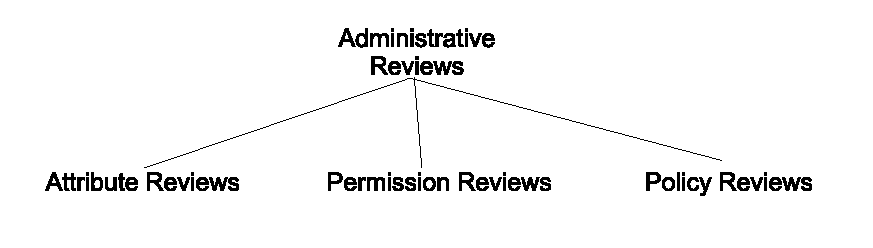
\includegraphics[width=.4\textwidth]{review-function-diagram}
		\caption{Review functions in ABAC}
		\label{fig:labac}
	\end{figure}
	

% Please add the following required packages to your document preamble:
% \usepackage{booktabs}
\begin{table}
	\centering
	\caption{Some review questions on an ABAC model} %\vspace*{3pt}
	\label{tab:review-functions-example}
	\begin{tabular}{|l|}						
		\hline					
		\multicolumn{1}{|c|}{\underline{\textit{I. Attribute Reviews }}}\\				 
		
			 1. What attributes are assigned to a user? \\
			 2. What are the values of a user attribute for a given user? \\
			 3. Which users are assigned to a given (attribute, value) pair? \\
			 4. Values of an object attribute? \\
			 5. What objects are assigned to a (attribute,value) pair ? \\
			 
		\multicolumn{1}{|c|}{\underline{\textit{II. Permission Reviews}}} \\		
		
	     	1. What permissions a user has? \\
	     	2. What permissions a user gains or looses after being assigned  \\ \hfil to a new attribute value? \\	     	 
	     	3. For a  certain permission, which attribute, values are required? \\
	     	
		\multicolumn{1}{|c|}{\underline{\textit{III. Policy Reviews}}} \\
		
			 1. Which users are allowed by a given policy? \\
			 2. Which objects are allowed by a given policy? \\
			 3. Which actions are granted by a given policy?\\
			 4. Which users (in term of (attribute, value) pair) are granted \\ \hfil what actions  on which objects (in term of (attribute, value) pair)?
		\\ \hline	
	\end{tabular}	
\end{table}


In addition to reviews on attributes, we can also pose interesting review questions on policies. While, some review questions may need to consider all  available policies in the system, some other simple reviews can be answered using a candidate policy. For simplicity, in this section, we are interested only on those simple review functions. Informally, let us assume an ABAC policy that says `users with clearance manager can approve existing loan' for user attribute `clearance' and value from the set \{manager, employee\}, object attribute `loan' and value from the set  \{existing, default\} and  and action 'approve'. Some simple review questions that we can ask using this policy include - a. who can approve existing loans ? b. which type of loan a manager can approve? c. who can approve which loans so on.

To formally define review functions, in the following section we first define a simple ABAC model - \sABAC{}. We follow the conventional approach for designing policies based on flexible policy language. In Section \ref{sec:review-function}, we define review functions using the \sABAC{} model. In Section \ref{section:np-complete}, we show that even simple policy review in \sABAC{} is NP-Complete. 

	
\newcommand{\phiu}{\phi_{u}}
\newcommand{\phio}{\phi_{o}}
\newcommand{\phia}{\phi_{a}}
\newcommand{\phip}{\phi_{p}}
\newcommand{\phix}{\phi_{x}}
\newcommand{\phiy}{\phi_{y}}
\newcommand{\userAttrExpr}{UAExpr}
\newcommand{\objectAttrExpr}{OAExpr}
\newcommand{\actionExpr}{AExpr}
\newcommand{\review}{acting\_users}
\newcommand{\simpleReview}{deep\_review}
\newcommand{\isSatisfiable}{is\_satisfiable}
\newcommand{\interpretationY}{I_y}
\newcommand{\interpretationX}{I_x}
\newcommand{\interpretation}{I}
\newcommand{\reductionAlgo}{CircuitSAT2PolicyReview}
\newcommand{\psiu}{\psi_{u}}



\subsection{\sABAC{} as a Conventional ABAC Model}
\sABAC{} model is defined for a finite set of users $U$, objects $O$ and actions $A$. Additionally, it has a set of attribute functions for users and objects. One or more user attributes form UAExpr, one of more object attributes form OAExpr and oen or more actions from AExpr.

	
\newcommand{\policyEval}{\delta}
% Please add the following required packages to your document preamble:
% \usepackage{booktabs}
\begin{table*}
	\centering
	\caption{  \sABAC{} Model} %\vspace*{3pt}
	\label{tab:labac-definition}
	\begin{tabular}{|l|}						
		\hline					
		\multicolumn{1}{|c|}{\underline{\textit{I. \sABAC{} Model } } }\\	
		
	 	- $U, O, A$: set of users, objects and actions \\
	 	- $UA,OA$: set of attribute functions for users and objects respectively.   \\ \hfill	$for_{ua \in UA}, ua: U \to 2^{range(ua)} $ and
	 	$for_{oa \in UA}, oa: O \to 2^{range(oa)} $ \\
	 	- policy: for an action, a policy $\phi_a$ is defined as shown in table \ref{tab:sabac-def}\\
	 	%-  policy: For an action a, a policy \phi_a is defined as shown table ?? \\
	 	 
	 
	 \hline	
	\end{tabular}
	
\end{table*}

%mod

	\newcommand{\UAttrVal}{\text{UAttrVal}}
\newcommand{\OAttrVal}{\text{OAttrVal}}
\newcommand{\Action}{action}
\newcommand{\E}{E}
% Please add the following required packages to your document preamble:
% \usepackage{booktabs}
\begin{table}[]
\centering
\caption{Policy Definition for \sABAC}
\label{tab:sabac-def}
\begin{tabular}{@{}l@{}}
 \hline
	$\phi ::= \phi \land \phi | \ \phi \lor \phi | \ (\phi) | \neg \phi $\\
 
	$\phi ::= \E $ \\
	Terminal Symbols:\\
	$ \E (attr: UA \cup OA, val: range(Attr))$ \\ \hfill  $\to \{true, false\}$ \\
	%$Act(\requestContext, a) \to \{true, false\}$\\
 %\bottomrule
 \\\hline
\end{tabular}
\end{table}

 
	


\subsection{Review Functions in \sABAC{}}
	

\textbf{Interpretation of Attribute Expression}\\
	Informally, an interpretation of an attribute expression  is the set of  $(attr,Value)$ pairs where $attr \in UA \cup OA$ and $Value \subseteq Range(attr)$ for which the attribute expression is evaluated to be true. Formally, we define interpretation as a function $\interpretation$ as follows.

\begin{itemize}
	\item $\interpretation(\phi) \to 2^{(attr: UA \cup OA,  Value: 2^{Range(attr)})}$ and  defined as \\
	$\interpretation(\phi) = \{(attr,Value) | (E(attr,val) \implies true ) \implies (\phi \implies true) \land val \in Value \}$
	
\end{itemize}
	
\noindent \textbf{Example of \sABAC{} Policy and its interpretation} \\
let $ \phi  \equiv \{ E(role, manager) \land \lnot E(role, dir) \land E(type, new) \}$ be a  \sABAC  policy. 	
$I_\phi = \{ (role,  \{ manager\}),$  $(type, \{ new\}), $   $(action, \{ approve\}) \}$ is satisfying interpretation for $\phi $. but $\{ (role,  \{ manager, dir\}) , (type, \{ new\}),$ \\ $(action, \{ approve\}) \}$ is not a satisfying interpretation. \\

\noindent \textbf{Review Function As a Decision Problem}
	
$\simpleReview=\{  \phi$ | exists an assignment of user and object attribute values of policy $\phi$ st. $\phi$ is evaluated true \}  \\
	
%Finally, we define review function $\reviewFunction$ as follows.$R(\phi, input:2^{\interpretation_\phi}) \to 2 ^{\interpretation_\phi}$, defined as  $R(\phi, input) = 2^{\interpretation_\phi} \setminus input$ \\	\\



 
 
% % Please add the following required packages to your document preamble:
 % \usepackage{booktabs}
 \begin{table}
 	\centering
 	\caption{Some review functions for \sABAC{}}
 	\label{tab:review-fun}
 	\begin{tabular}{|l|l|l|}
 		 \hline
 		 \textit{function Name} &  \textit{Input} &  \textit{Output}\\
 		 \hline
 		 \textit{\request} &   \{$\interpretation(\phiu), \interpretation(\phio), \interpretation(\phia)$\}&  $\delta \equiv \{true, false\}$ \\ 		 
 		 
 		 \hline
 		 \textit{UA-query} &   \{$ \interpretation(\phio), \interpretation(\phia), \delta$\}&  $\{\interpretation(\phiu)\}$ \\
		\hline
		\textit{OA-query} &   \{$ \interpretation(\phiu), \interpretation(\phia), \delta$\}&  $\{\interpretation(\phio)\}$ \\
		\hline
		\textit{Act-query} &   \{$ \interpretation(\phiu), \interpretation(\phio), \delta$\}&  $ \{ \interpretation(\phia) \}$ \\
		\hline
		\textit{UO-query} &   \{$ \interpretation(\phia), \delta$\}&  $ \{ \interpretation(\phiu),\interpretation(\phio) \}$ \\
			\hline
		\textit{deep-query} &   \{$\delta$\}&  $ \{ \interpretation(\phiu),\interpretation(\phio),  \interpretation(\phia),  \}$ \\
			\hline
 	\end{tabular}
 \end{table} 
 

  \subsection{Policy review in \sABAC{} is NP-Complete }
	
	we first informally argue that there exists a one-to-one correspondence between a boolean circuit and a policy in \sABAC{} model. Roughly, a boolean circuit is composed of n boolean variables/inputs (each denoted by $x_i$ and having a value from $\{0, 1\}$ )   and one boolean output ($y$) (in general, m outputs. But for our purpose we stick to one output). On the other hand, a \sABAC{} policy is composed of one or more functions of  $E$ which is also evaluated to be either true and false.  While boolean variable uses AND, OR and NOT gates, \sABAC{} policies uses logical $\land, \lor, \lnot$ respectively which corresponds semantically. Analogous to the output of a boolean circuit, evaluation of an \sABAC{} policy is either true or false. Thus we say a boolean circuit and a \sABAC{} policy correspond to each other. 
	
	Satisfiability of a boolean circuit asks for values of each boolean variable, $x_i$ that make the output of the circuit to be one. Similarly,  a review function (for example, in deep_review in Table \ref{table:review-fun}) may ask for possible attribute value assignments that evaluates  a access control request to be true. 
	%Each input ($x_i$) in the boolean circuit, can be thought of a evaluation function ($E$) in the UAExpr and OAExpr. \sABAC 
	
	 \subsubsection{CircuitSAT}
	 

\begin{table}[]
	\centering
	\caption{Boolean Circuit }
	\label{my-label}
	\begin{tabular}{@{}l@{}}
		\toprule
		$\psi ::= \psi \ AND \  \psi | \psi \ OR \  \psi | (\psi) | \ NOT \ \psi $ \\
		 $ \psi ::= x_i$ \\
		Terminal Symbols \\
		$x_i \in \{true, false\} $  \\		
		\bottomrule
	\end{tabular}
\end{table}

\noindent $\CircuitSAT = \{ \psi |$ there exists truth value assignments of each input $x_i$ that satisfy the boolean circuit $\psi$\} \\

	 

	
	 \textbf{NP Completeness of Policy Review} 
\begin{itemize}
	\item $\simpleReview \in NP$
		 given an instance of \simpleReview,   $\phi$  and a certificate $\interpretation$ for $\phi$. We can verify the certificate by evaluating each function $\E \in \phi$ with given attribute and values in $\interpretation$ in linear time. 
		
	\item Algorithm \ref{alg:reduction}  reduces \CircuitSAT{} to \simpleReview

	\item $\psi \in \CircuitSAT \implies \reductionAlgo(\psi) \in \simpleReview$:
		    $\psi  \in \CircuitSAT$ means there is a satisfying assignment of all $x_i \in \psi$. We replace all boolean variable, $x_i$ with evaluation function, $E_i$ resulting $\psiu$. So there must be a satisfying truth assignment of each $E_i$ satisfying $\psiu$. If we use the same (attribute, value) pairs as used in the construction of each $E_i$, we get a satisfying interpretation of attributes, $\interpretationX$ for $\psiu$.
		     %As a result, for $(\psiu \land \E(a_i, val_i), E(a_i, val_i), ( ai, \{val_i\}) )$, there is an interpretation $\interpretationX$ that satisfy $\psiu$. That means, $\reductionAlgo(\psi) \in \simpleReview$. ( because of fact that  $\reductionAlgo(\psi)$ results $(\psiu \land \E(a_i, val_i), E(a_i, val_i), ( ai, \{val_i\}) )$)
	\item $ \phi \in \simpleReview \implies \exists \psi [ \psi \in \CircuitSAT]$:	\\
		   If we replace each $\E_i$ in $\phi$ with $x_i$ resulting $\psi$, $psi$ is still satisfiable because $\phi$ is satisfiable. This implies that $\psi \in \CircuitSAT$. 
		
	\item Algorithm \ref{alg:reduction} runs in polynomial time. 
\end{itemize}
	
	
	\begin{algorithm}
	\caption{ Reduction of Circuit SAT to Policy Review Problem}
	\label{alg:reduction}
	\begin{algorithmic}[1]
		\Procedure{\reductionAlgo ($Circuit \ \psi$)}{}
		\State Replace boolean ops with logical ops.
		\For{each variable  $x$ \Pisymbol{psy}{206} $\psi$ }
		\State replace $x$ with \textbf{\E($a \in UA \cup OA, val \in range(a)$) } 
		\EndFor
		\State let $\psiu$ denote the resulting \userAttrExpr		
		\State return $\psiu$ 	
		\EndProcedure
	\end{algorithmic}
\end{algorithm}

\subsubsection{Policy Review in LaBAC is Polynomial}
% %\newcommand{\E}{E}
% Please add the following required packages to your document preamble:
% \usepackage{booktabs}
\begin{table} 
\centering
\caption{Policy Definition for \elabac{}}
\label{table:sabac-def}
\begin{tabular}{@{}l@{}}
 \toprule	
	$\phi ::= \phi \land \phi  $\\
	$\phi ::= \E $ \\	 
	Terminal Symbols\\
	$ \E (label: UA \cup OA, val: range(label) \cup NUL \cup NOL)  \to$ \\ \hfill $\{true, false\}$ \\
 \bottomrule
\end{tabular}
\end{table}